The problem visualisation was implemented as an application using the R-Shiny framework, which consists of three components: a user interface object, a server function and a call function. The code for each component can be found in the appendix.\\

\noindent Essentially the \hyperlink{call function}{call function} just specifies which user interface object and server function to call in the Shiny app.

\bigskip

\subsection{User interface}

\noindent The \hyperlink{User interface}{user interface object} consists of three tabs. The default tab shows the description of the problem, similar to the introduction to this thesis.\\

\begin{figure}[h!]
    \centering
    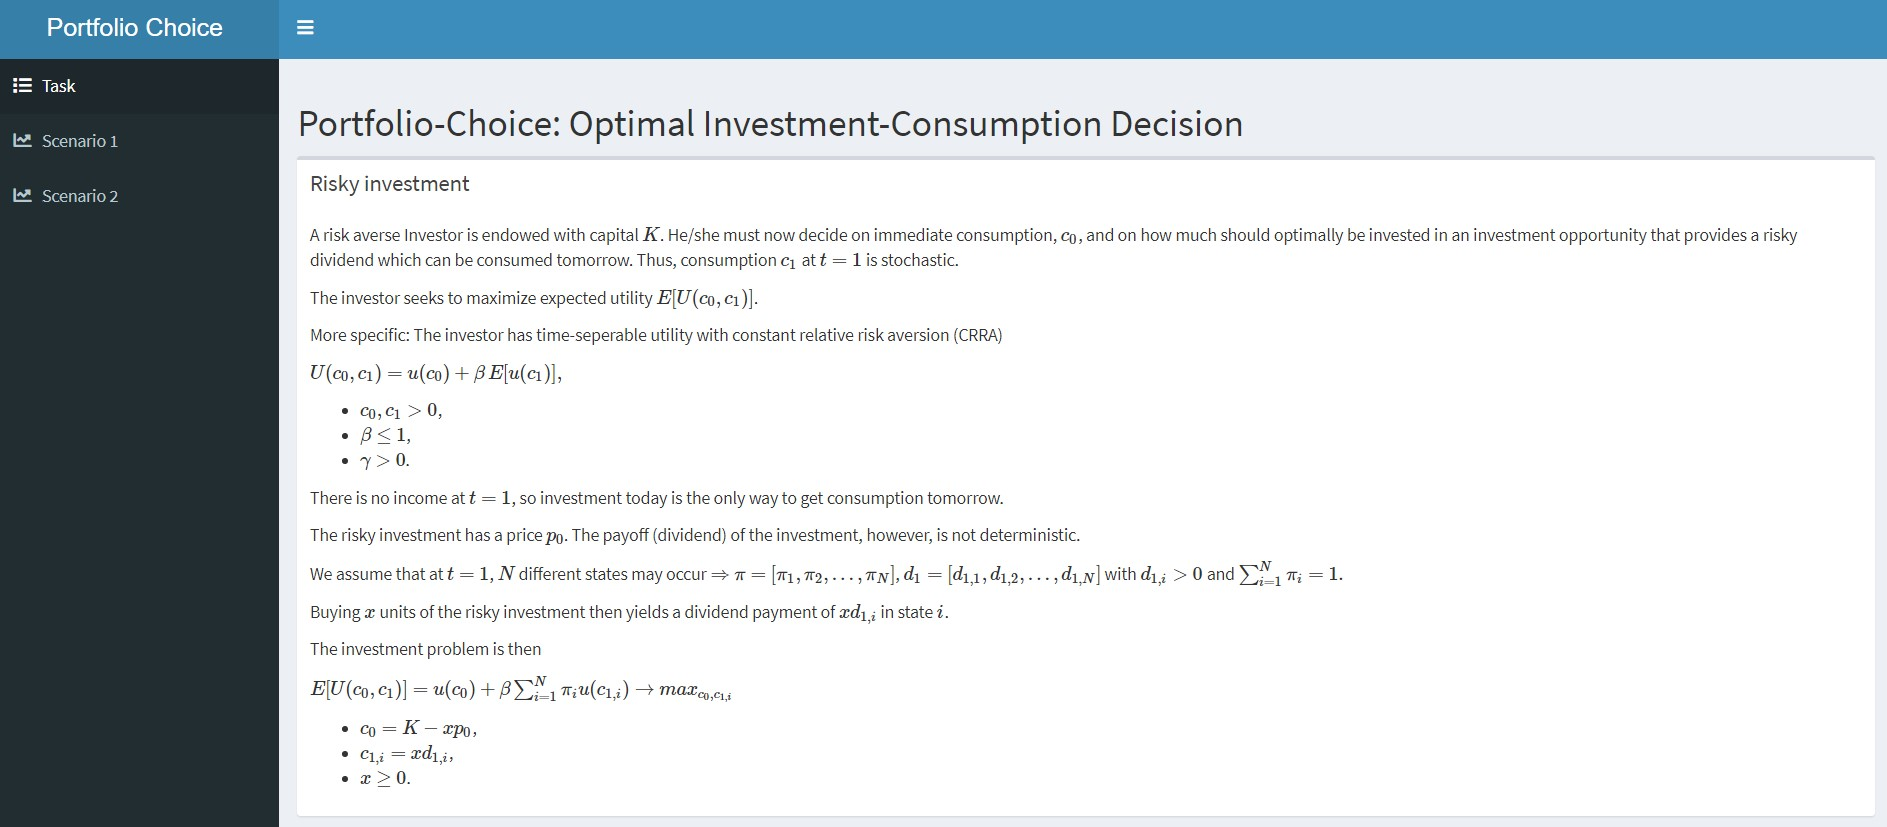
\includegraphics[width=0.7\textwidth, trim = 0 0 0 0,clip]{files/1.1.jpg}
    \caption{Problem description}
\end{figure}

\bigskip

\noindent The second tab is the visualization of the first scenario: The top diagram shows a plot of the utility generated at $t=0$, the expected utility in $t=1$ and the total expected utility.\\
Secondly, a diagram of indifference curves is displayed.\\
Finally, there is a plot of the total expected utility and the marginal utility. \\
All parameters can be set individually by the user. For this purpose, there are sliders on a panel on the left side. There are also two reset buttons, one for the function parameters and one for the investment parameters. At the bottom of the panel, the values of the resulting optimum are displayed.\\
The visualization of scenario 2 is located on the third tab, which is structured analogously.

\bigskip

\subsection{Server function}

\noindent The \hyperlink{Server function}{server function} can be divided into two parts. Up to line 448 the functions for scenario 1 are defined, afterwards the functions for scenario 2. Both parts are once again similar in structure:\\

\noindent First, the function and the default values for the reset buttons are set. In the code, this is done from line 3 to line 79 for scenario 1 and from line 466 to 550 for scenario 2.\\

\noindent From line 80 to 130 and line 551 to 599, respectively, the function comes, which adjusts the probabilities so that the sum always adds up to 100\%.\\

\noindent Between line 131 and 157 and line 600 and 629, respectively, the function parameters and investment specifications are imported and collected into lists for easier processing.\\

\noindent Then, in line 158-187 for scenario 1 and line 630-667 for scenario 2, respectively, the function follows, which maximizes the utility function. It is assumed that the constraints \eqref{eq:scenario1_constraints} and \eqref{eq:scenario2_constraints}, respectively, are binding. In section 4.1 and section 4.2 it is shown that in the optimum this must be true.\\
For simplicity, the utility function is evaluated on a discrete set of points and the maximum can easily be determined. Since the utility function in scenario 1 is one-dimensional, evaluation over a vector is sufficient to find the optimal investment $x^*$. In Scenario 2, the utility function is evaluated over a matrix in order to find the best combination of $x$ and $y$, which is denoted as $(x^*, y^*)$.\\

\noindent Between line 188 and 250 and line 668 and 771, respectively, the charts are generated: For Scenario 1, the first diagram simply consists of the three graphs, total utility, utility at $t=0$ and expected utility at $t=1$, plotted over the amount spent on the risky investment $xp_0$. The diagram for scenario 2 consists of two separate plots. First, the graphs are plotted over $xp_0$ while $yb_0$ remains fixed at $y^*b_0$ and then vice versa.\\

\begin{figure}[h!]
  \centering
  \begin{minipage}[b]{0.44\textwidth}
    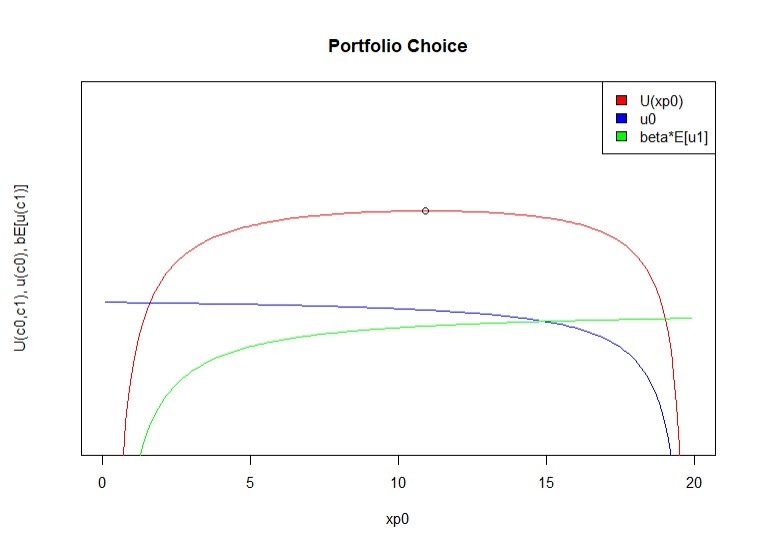
\includegraphics[width=\textwidth, trim = 10 0 30 40,clip]{files/2.1.jpg}
    \caption{Utility, scen. 1}
  \end{minipage}
  \hfill
  \begin{minipage}[b]{0.53\textwidth}
    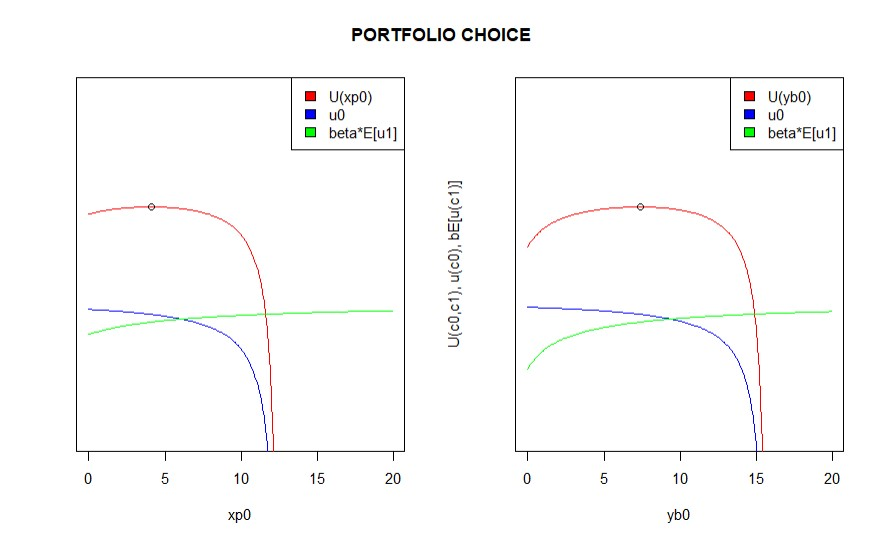
\includegraphics[width=\textwidth, trim = 10 0 20 40,clip]{files/3.1.jpg}
    \caption{Utility, scen. 2}
  \end{minipage}
\end{figure}

\bigskip

\noindent From line 251 to 340 and line 772 to 881, respectively, follows the generation of the plot of indifference curves. The abscissa corresponds to $xp_0$, i.e. the amount of capital spent on the risky investment. The ordinate refers to the amount consumed immediately, $c_0$. For one indifference curve, the constant value is equal to the utility generated in the optimum, which is the maximum possible utility with the given parameters and constraints. Meanwhile, the share of riskless invested capital remains fixed at $y^*b_0$. The other indifference curve can be chosen by the user by adjusting a slider. From then on, things work a little differently for scenario 1 and scenario 2:\\
In scenario 1, the user determines a certain percentage of the original capital. This proportion of capital is then added to (or subtracted from) the originally available capital. The constant value of the indifference curve then corresponds to the maximum utility possible with this newly available capital.\\
In scenario 2, the user determines how much more or less (in percent) is spent on the riskless investment. The budget constraint remains binding. Thus, the amount spent on consumption and the risky investment also changes, and the resulting utility cannot be the optimum. The constant value of the new indifference curve corresponds to the maximum possible utility at the given risk-free expenditure. All points $(xp_0, c_0)$ for which this holds are part of the indifference curve. The legend shows the resulting utilities for the two indifference curves and the amount spent on the riskless investment.\\

\begin{figure}[h!]
  \centering
  \begin{minipage}[b]{0.45\textwidth}
    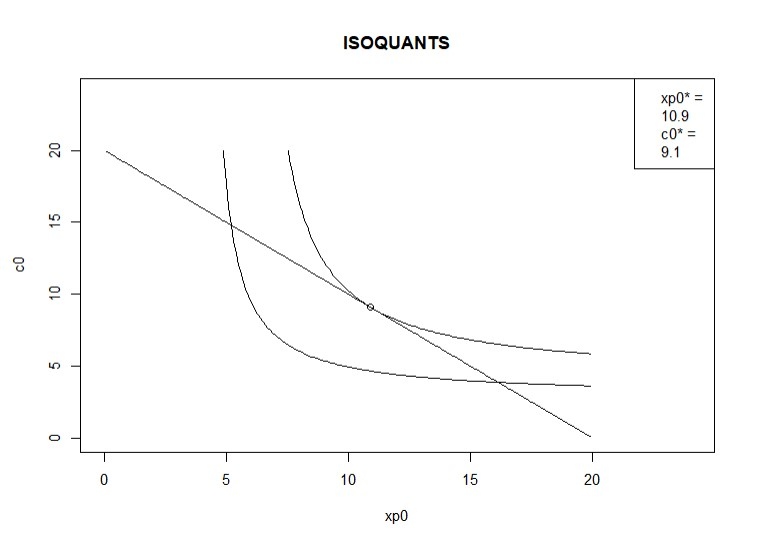
\includegraphics[width=\textwidth, trim = 0 0 0 40,clip]{files/2.2.jpg}
    \caption{Indifference curves, scen. 1}
  \end{minipage}
  \hfill
  \begin{minipage}[b]{0.53\textwidth}
    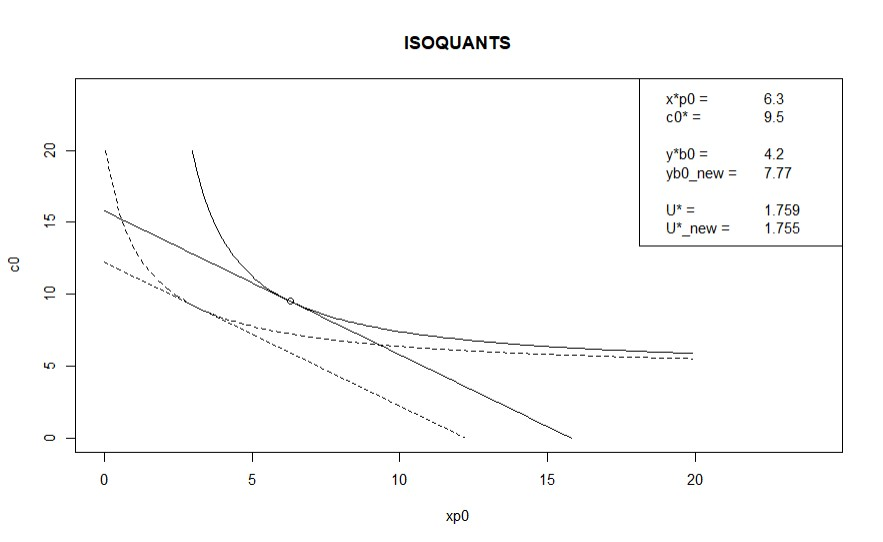
\includegraphics[width=\textwidth, trim = 0 0 0 40,clip]{files/3.2.jpg}
    \caption{Indifference curves, scen. 2}
  \end{minipage}
\end{figure}

\bigskip

\noindent The last diagram is generated between line 341 and 451 for scenario 1 and line 882 and 999. It shows in sub-diagrams the total expected utility plotted over $c_0$, $xp_0$ and $yb_0$, respectively, for scenario 2. The optimum is marked and the marginal utility is shown as a tangent through the optimum.\\

\begin{figure}[h!]
  \centering
  \begin{minipage}[b]{0.47\textwidth}
    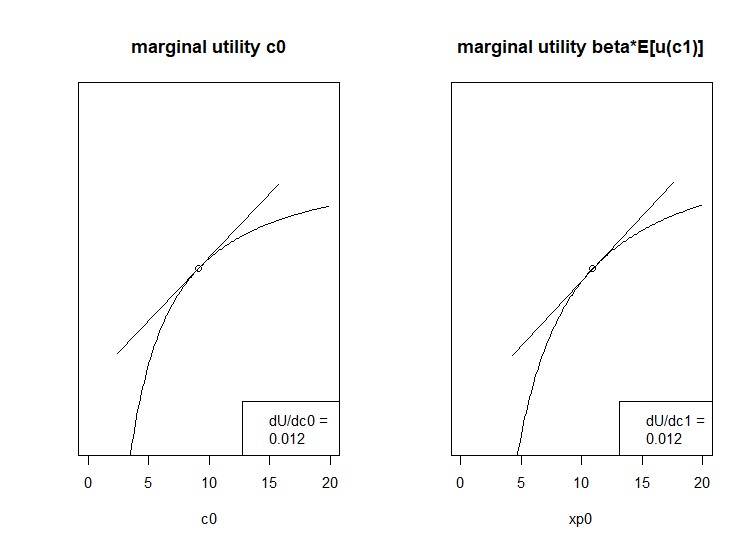
\includegraphics[width=\textwidth, trim = 0 10 0 36,clip]{files/2.3.jpg}
    \caption{Marginal utilities, scen. 1}
  \end{minipage}
  \hfill
  \begin{minipage}[b]{0.51\textwidth}
    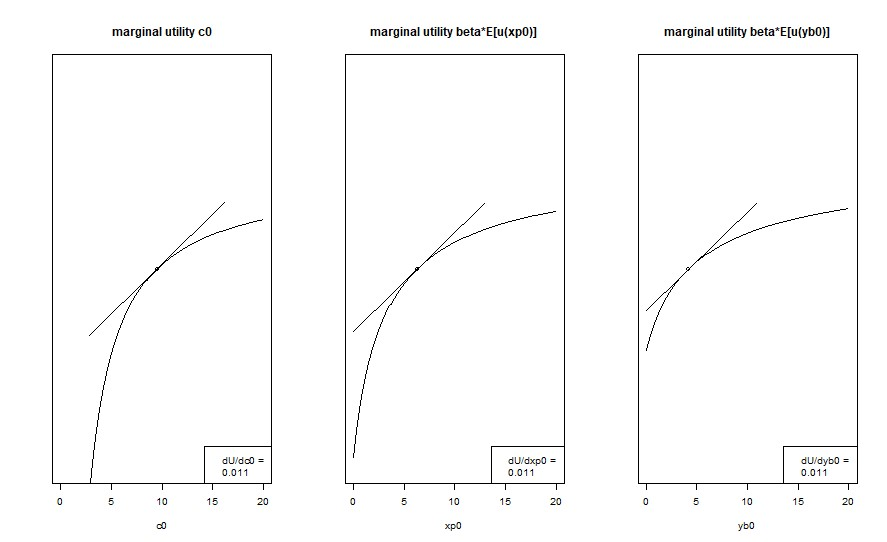
\includegraphics[width=\textwidth, trim = 0 0 0 32,clip]{files/3.3.jpg}
    \caption{Marginal utilities, scen. 2}
  \end{minipage}
\end{figure}

\bigskip

\noindent Finally (lines 452-465 and line 1000-1016, respectively), the function follows which gives the maximum expected utility, the amount consumed immediately and the expenditure on the investments at the optimum.
Small errors may occur, due to the discretization of the domain over which the optimum is evaluated.